\documentclass[../report.tex]{subfiles}
\begin{document}

\section{Combining the Designed Modules} \label{sec:combined}
The final block diagram implemented in VHDL is shown in \autoref{fig:combining:overview}.
\begin{figure}[H]
    \centering    
    \noindent\makebox[\textwidth]{%
    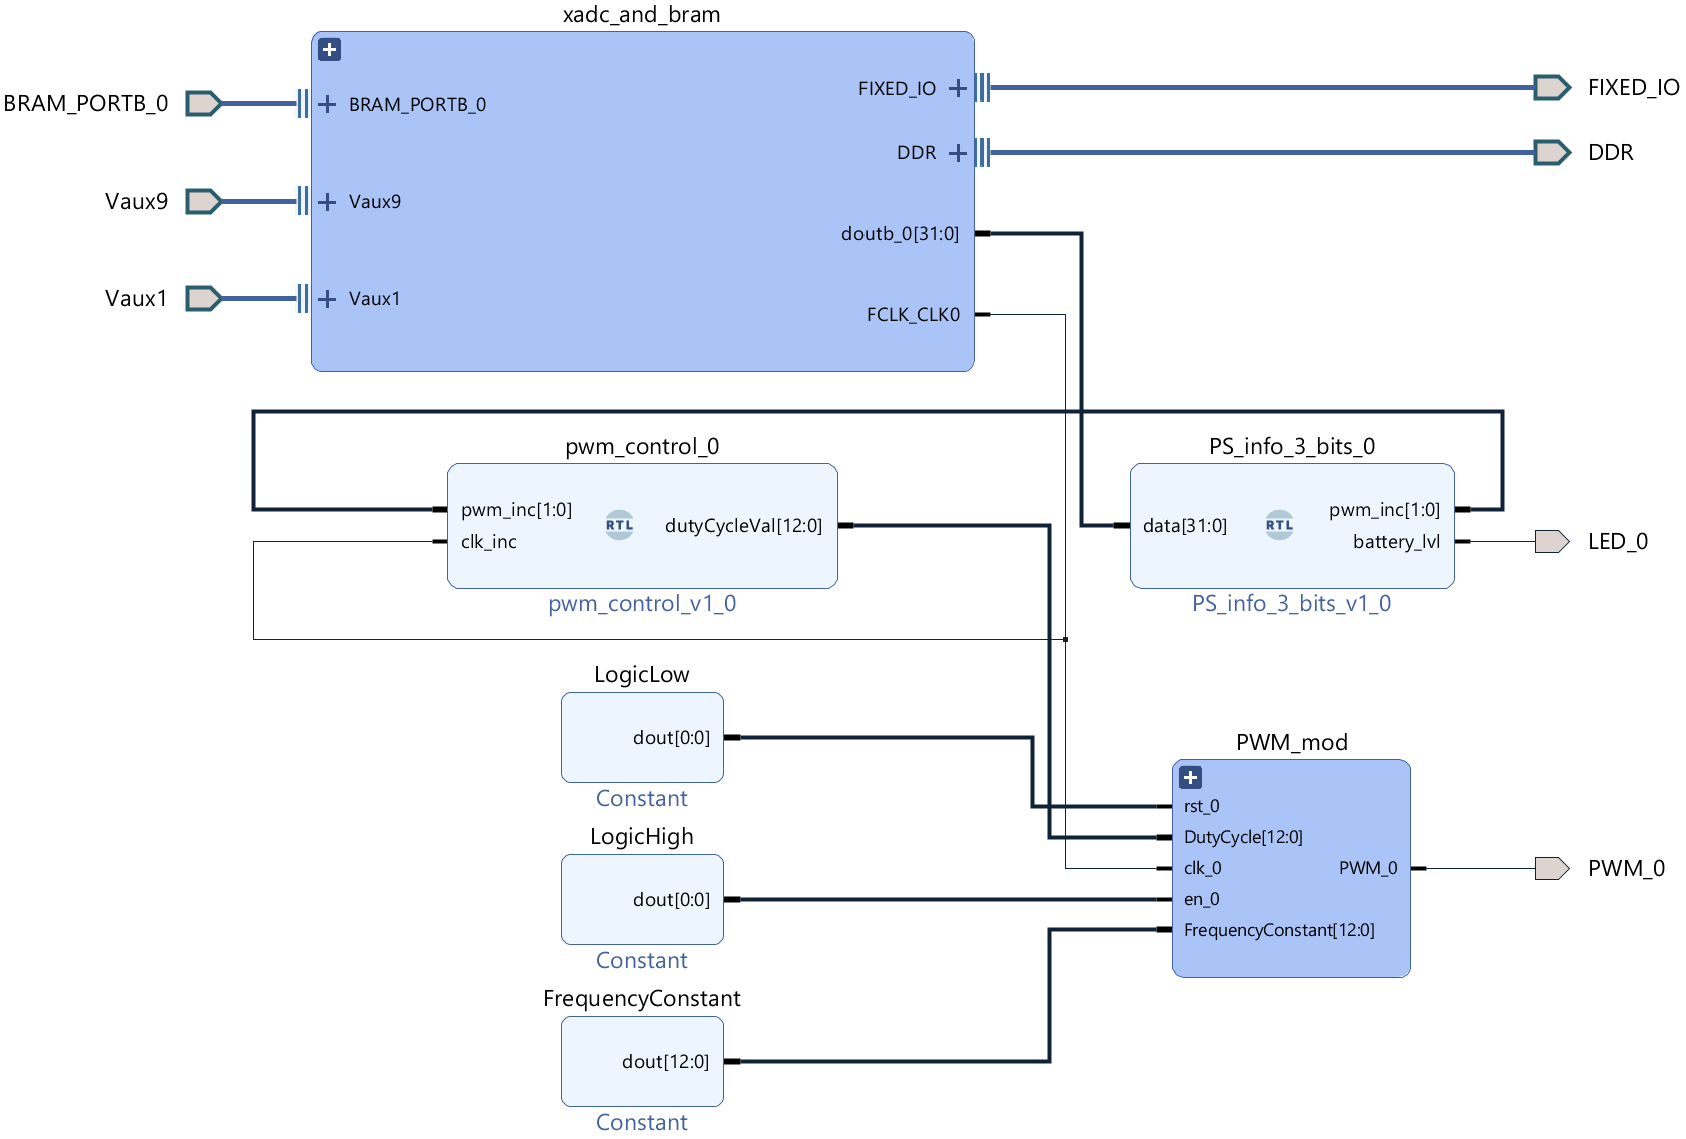
\includegraphics[width=1.2\textwidth]{figures/diagram/system_block.png}}
    \caption{Block diagram of the final product implemented in VHDL.}
    \label{fig:combining:overview}
\end{figure}
The \texttt{PWM\_0} pin is mapped to an external pin and attached to the charging circuit. The pin \texttt{LED\_0} is attached to a LED through the constraint file, to show when the battery percentage is above 20 \%. The circuit's $V_{ADC1}$ and $V_{ADC2}$ is connected to \texttt{Vaux1} and \texttt{Vaux9}, through a mapping in the constraint file.\\

The block \texttt{pwm\_control\_0} is used as a layer between the PWM module and the reading of PWM command. This module increases, decreases or keeps the duty cycle constant, which is used for the module \texttt{PWM\_{mod}}.

\end{document}